\documentclass[11pt,a4paper,utf8x]{report}
\usepackage[T1]{fontenc} 
\usepackage[utf8]{inputenc} 
\usepackage{lmodern}
\usepackage [frenchb]{babel}
% Pour pouvoir utiliser 
\usepackage{ucs}

\usepackage{textcomp}
\usepackage{graphicx}
\usepackage{keystroke}
\usepackage{amssymb}
\usepackage{amsmath}
\renewcommand{\thesection}{\arabic{section}} % numérotation des sectiosn
\usepackage[cc]{titlepic} %rajouter le logo dans la page de garde
\usepackage{url} % Pour avoir de belles url
\usepackage {geometry}
\usepackage[linktocpage]{hyperref}
% Pour pouvoir faire plusieurs colonnes
\usepackage {multicol}
%Pour faire plusieurs lignes
\usepackage{multirow}
\usepackage{slashbox}
% Pour mettre du code source
\usepackage {listings}
% Pour pouvoir passer en paysage
\usepackage{lscape}	

% Pour pouvoir faire plusieurs colonnes
\usepackage {multicol}

% POur crééer un index
\usepackage{makeidx}


\usepackage{pdfpages}

\hypersetup{
backref=true,
%permet d'ajouter des liens dans...
pagebackref=true,%...les bibliographies
hyperindex=true, %ajoute des liens dans les index.
colorlinks=true, %colorise les liens
breaklinks=true, %permet le retour à la ligne dans les liens trop longs
urlcolor= blue, %couleur des hyperliens
citecolor=	cyan,
bookmarks=true, %créé des signets pour Acrobat
bookmarksopen=true,
%si les signets Acrobat sont créés,
%les afficher complètement.
pdftitle={Initiation à la Recherche}, %informations apparaissant dans
pdfauthor={MARGUERITE Alain\\ RINCE Romain},
%dans les informations du document
pdfsubject={Doc}
%sous Acrobat.
}

\makeindex


%%%% debut macro pour enlever le nom chapitre %%%%
\makeatletter
\def\@makechapterhead#1{%
  \vspace*{50\p@}%
  {\parindent \z@ \raggedright \normalfont
    \interlinepenalty\@M
    \ifnum \c@secnumdepth >\m@ne
        \Huge\bfseries \thechapter\quad
    \fi
    \Huge \bfseries #1\par\nobreak
    \vskip 40\p@
  }}

\def\@makeschapterhead#1{%
  \vspace*{50\p@}%
  {\parindent \z@ \raggedright
    \normalfont
    \interlinepenalty\@M
    \Huge \bfseries  #1\par\nobreak
    \vskip 40\p@
  }}
\makeatother
%%%% fin macro %%%%

%Couverture 

%Couverture 

\widowpenalty=10000
\clubpenalty=10000
 
\title{ \huge{Initiation à la Recherche \vspace{3cm} }% \\ \emph{Conception et réalisation d’un logiciel interactif de visualisation de pavages 2D/3D }%\vspace{3cm}
}

\titlepic{
\includegraphics[scale=0.80]{img/logolina}     \hspace{2cm} 
\includegraphics[scale=0.80]{img/logouniv}}


\author{A.\textsc{Marguerite}\\ R.\textsc{Rincé}}%\vspace{3cm}}
\date{Université de Nantes \\ 2 rue de la Houssinière, BP92208, F-44322 Nantes cedex 03, FRANCE}
%\vspace{20cm}
% Nice RRealpaver
\newcommand{\realpaver}{\emph{Realpaver}}


%\vspace{9cm}
\date{Université de Nantes \\ 2 rue de la Houssinière, BP92208, F-44322 Nantes cedex 03, FRANCE}
%\vspace{20cm}

\hyphenation{vi-sua-li-sa-tion}
\hyphenation{vi-sua-li-sé}
\hyphenation{vi-sua-li-sée}
\hyphenation{vi-sua-li-sés}
\hyphenation{vi-sua-li-sées}
\hyphenation{si-tu-a-tion}
\hyphenation{a-na-lyse}

\begin{document}

\maketitle
\renewcommand{\labelitemi}{$\bullet$} 

\clearpage

\tableofcontents
\clearpage


\chapter{Introduction}

\section{Présentation du sujet}
Le module \emph{Initiation à la recherche} du 2\up{nd} semestre du master \textsc{ALMA} propose une initiation au métier de chercheur en informatique. Dans le cadre de ce module notre binôme a choisi le sujet : \emph{Conception et réalisation d’un logiciel interactif de visualisation de pavages 2D/3D}. Ce sujet à la particularité d'être la reprise d'un projet de stage. Ce stage effectué au cours de l'été 2011 par un membre du binôme avait pour objectif initial la conception et la réalisation d'un outil de visualisation des calculs en sortie du logiciel  \realpaver (cf. \ref{realp}) développé au sein de l'équipe d'accueil. Le développement de ce stage a suivit le modèle du cycle en V décrit par la figure \ref{fig:vcycle}.
\begin{figure}[htbp]
\centering
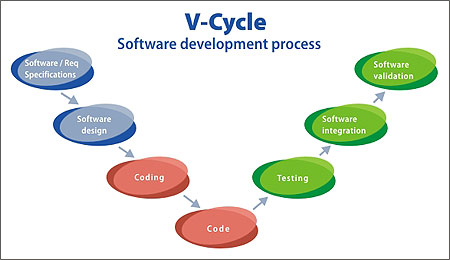
\includegraphics[scale=1]{img/vcycle}
\caption{Cycle en V}
\label{fig:vcycle}
\end{figure}
\clearpage
Au terme des deux mois de stage, le travail accompli fut le suivant :
\begin{enumerate}
\item 
Rédaction du cahier des charges (cf. \ref{sec:cac}).
\item
Rédaction du document de spécification (cf. \ref{sec:spe}).
\end{enumerate} 

\section{\'Equipe d'accueil}
L'équipe Optimisation globale, optimisation multi-objectifs\cite{opti} (\textsc{OPTI}) du laboratoire \textsc{LINA}\cite{lina} travaille principalement sur des méthodes visant à la résolution efficace de problèmes d’optimisation complexes.  
\section{Déroulement du projet}
Au cours des premières semaines, C.\textsc{Jermann} nous a proposé d'étudier de manières générales les sujets de l'équipe \textsc{OPTI}. Un bref bilan de cette étude est proposé dans le chapitre \ref{chap:doc}. En parallèle, nous avons manipulé quelques outils ad-hoc tel que gnuplot \cite{gnu}, utilisés jusqu'à présent par l'équipe \textsc{OPTI} pour représenter les valuations calculées par \realpaver. Par la suite nous avons pris (ou repris) connaissance du cahier des charges et du document de spécifications, en apportant certaines corrections à ce dernier. 

\paragraph{}Une problématique est apparue quant à l'axe d'étude à choisir pour le déroulement du projet. En effet une des caractéristiques principale de l'outil à concevoir, est de manipuler un nombre potentiellement très grand de données (cf. \ref{chap:con}). Nos alternatives étaient alors les suivantes : 
\begin{enumerate}
\item
Étudier les différents algorithmes et structures de données nécessaires à l'outil.
\item
Entamer directement la conception de l'outil (choix de design pattern, IHM, \dots).
\end{enumerate} 
Ce second choix impliquait la possibilité au terme de l'année, de proposer un résultat «matériel». En effet le document de spécifications étant très concis, nous aurions pu très rapidement produire du code en le suivant à la lettre. Cependant cette démarche ne répondait pas aux objectifs de découverte du module d'Initiation à la Recherche. De plus, passer outre cette étude de structures et d'algorithmes, aurait rapidement entraîné la conception dans une impasse. Nous avons donc choisi la seconde alternative. Notre contribution à cette étude est résumé dans le chapitre \ref{chap:con} de ce document.


\chapter{Rapport de documentation}\label{chap:doc}
\section{Introduction }
%Dans le cadre du module Initiation à la recherche, 
L'objectif de ce document est de décrire les notions essentielles à retenir en ce début de projet d'initiation à la recherche. Ces notions font partie d'un même sujet d'étude, au cœur des travaux de l'équipe \textsc{OPTI}. Elles concernent le sujet des contraintes et des intervalles. %Aussi des notions d'optimisation seront abordées.

\section{Présentation du problème}
\subsection{Définition du contexte}
Un problème de satisfaction de contraintes (\textsc{CSP}) est défini par 3 éléments : 
\begin{itemize}
\item
Un ensemble de variables $\mathbf{V} = \left\{ v_1,...,v_n \right\}$.
\item
Un domaine de valeurs pour chaque variable. Chaque valeur du domaine $D_i$ associé à la variable $v_i$ est une valeur que peut potentiellement prendre $v_i$ : $\mathbf{D} = D_1 \times ... \times D_n $.
\item
Un ensemble de contraintes (relations) $\mathbf{C}$ restreignant les variables de $\mathbf{V}$ défini ci-dessus :  $\mathbf{C} = \left\{c_1,...,cm\right\}$. 
\end{itemize}
\vspace{1.5cm}
On s'intéressera notamment à la résolution des \textsc{CSP} sur le domaine continu. Dans ce cas les domaines des variables seront des intervalles dans les réels et les contraintes seront généralement représentées par des équations et des inégalités. 

%\clearpage
\subsection{Exemple}

Une représentation simple de ce type de problèmes est la recherche des intersections de deux cercles dans un plan. Définissons deux cercles respectivement de rayons  $r_1$ et $r_2$ et de centres : $(x_1,y_1)$ et $(x_2,y_2)$.
On peut alors fixer les données en entrées du problème :

\begin{itemize}
\item
Un ensemble de variables $\{x,y\}$ .
\item
Un domaine de valeurs pour chaque variable. 
\item
Les constantes du problème : les rayons de chaque cercle situés dans  $\mathbb{R⁺}$.
\item
L'ensemble des contrainte est composé par les équations des cercles :
\begin{equation}\label{eq}
\begin{cases}
(x-x_1)²+(y-y_1)² = r_1²\\
(x-x_2)²+(y-y_2)² = r_2²
\end{cases}
\end{equation}
\end{itemize}


\section{Méthodes de calculs}
Les méthodes de calculs permettent la résolution de problèmes mathématiques en machine; en particulier lorsque l'on cherche à résoudre des problèmes sur les nombres réels. Elles permettent par exemple la résolution des \textsc{CSP}  ou \textsc{GCSP} (Geometric Constraint Satisfaction Problem \cite{Jermann}) et peuvent être divisées en deux catégories : les méthodes formelles et les méthodes numériques.


\subsection{Méthodes formelles}
Les méthodes formelles permettent de résoudre des systèmes d'équations ou d'inéquations en utilisant au maximum le calcul symbolique. Les approches les plus classiques des méthodes formelles utilisent des théories, telles que les idéaux polynomiaux pour les bases de Gröbner, ou la théorie des déterminants pour la méthode du résultant.

 Ces méthodes ont l'énorme avantage de retourner des solutions exactes d'un système d'équation, ou tout du moins de minimiser l'utilisation de l'arithmétique flottante. Elles tenteront donc de résoudre le problème \ref{eq} en effectuant uniquement des opérations sur les équations sans évaluer les variables. On pourra donc avoir des expressions pour $x$ et $y$ représentant les solutions du problème de façon symbolique. 

Cependant les résolutions de problèmes par des méthodes formelles sont forcément restreintes par les possibilités du calcul symbolique et ne pourront donc pas toujours offrir de solution générale et met en œuvre des algorithmes de complexité exponentielles. Il n'existe par exemple pas de formules générales permettant de trouver les solutions d'un polynôme de degré supérieur ou égal à cinq.


\subsection{Méthodes numériques}
Les méthodes numériques consistent à évaluer de façon calculatoire la ou les solutions d'un problème. En effet elles sont capables d'essayer de résoudre n'importe quel système d'équation (ou d'égalités). Ainsi dans le cas du problème \ref{eq} la machine va affecter directement les calculs pour évaluer le résultats. Or l'utilisation de la représentation flottante et de son arithmétique pour simuler les opérations réelles va entrainer une diffusion et une augmentation de l'erreur de calcul, à tel point que l'on ne peut  parfois plus assurer la validité d'une solution. On pourra d'ailleurs citer à titre d'exemple le problème de l'inversion d'une matrice mal conditionnée\cite{Conditionnement}. 

Cependant ces calculs numériques utilisés  par des méthodes de résolutions par intervalles permettent de contourner ces problèmes. Pour plus de détails sur la représentation flottante, on pourra se référer à la thèse de Frédéric \textsc{Goualard}\footnote{Notamment dans la première Partie : \emph{Chapitre 1 : L’arithmétique flottante}} \cite{Goualard}.


\section{Résolution par Intervalles}
Les méthodes formelles et numériques, bien que performantes par certains aspects, sont rapidement limitées lorsque l'on veut résoudre des problèmes complexes ou que l'on veut pouvoir valider une solution (problème de propagation des erreurs\dots{}). C'est dans ce cadre que la méthode de résolution par intervalles a toute sa place. Construite grâce à l'arithmétique des intervalles, elle utilise aussi des notions apportées par la programmation par contraintes.
 
\subsection{L'Arithmétique des intervalles}
Cette arithmétique permet un calcul sur l'ensemble $\mathbb{I}$ des intervalles à bornes sur $\mathbb{R}$. Les bornes $b1$ et $b2$ de l'intervalle $[b1,b2]$, résultant de tout calcul, sont choisies en prenant un arrondi respectivement inférieur à $b1$ et supérieur à $b2$ de manière à garantir l'exactitude des calculs. L'extension des fonctions aux intervalles, introduite par \textsc{Moore} en 1966, permet une transition à des intervalles grâce à un opérateur d'encadrement. Les opérations élémentaires sont alors réécrites en terme des bornes des intervalles, par exemple : 

\begin{equation}\label{eq2}
\begin{cases}
[a .. b] + [c .. d] = [a + c .. b + d] \\
[a .. b] × [c .. d] = [min(ac, ad, bc, bd) .. max(ac, ad, bc, bd)]
\end{cases}
\end{equation}

Dans le cas d’une fonction non monotone comme le cosinus, on découpe les intervalles en domaines où la fonction est monotone  (\ref{fig:Cos})

\begin{figure}[h] %on ouvre l'environnement figure
  \center
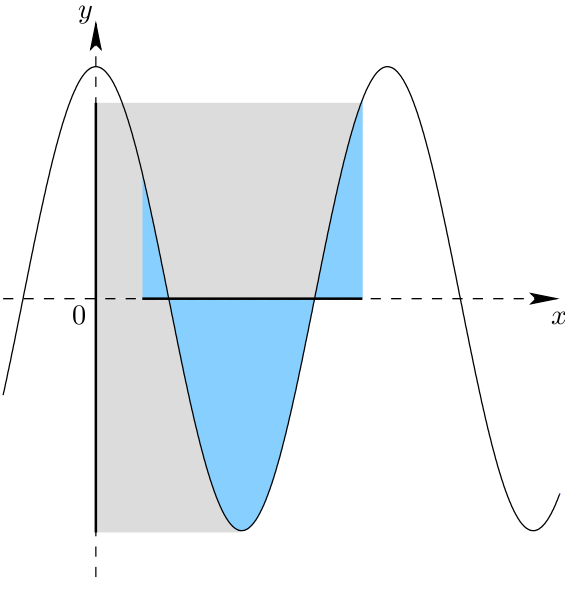
\includegraphics[scale=0.30]{img/cos}
  \caption{Cas de la fonction cosinus} %la légende
 \label{fig:Cos} %la légende
\end{figure} %on ferme l'environnement figure


Une liste non-exhaustive des opérations de cet opérateur est listée dans \cite{Goualard}.



\subsection{Utilisation des intervalles pour la notion de contraintes}
Également, la méthode de résolution par intervalles utilise des notions de programmation par contraintes. On y retrouve celle de consistance. La consistance consiste à rechercher les valeurs cohérentes dans le domaine des variables pour les contraintes du \textsc{CSP}. Par exemple un \textsc{CSP} est globalement consistant lorsque toutes les valeurs des variables de son domaine appartiennent au moins à une solution. On devine qu'il peut être intéressant pour un \textsc{CSP} de posséder la consistance la plus forte possible. Ainsi les opérations pour la résolution de problèmes seront moins nombreuses. %Cette méthode appliquée au problème d'intersection de deux cercles, illustre les solutions de la manière suivante   

%~ \begin{figure}[ht!] %on ouvre l'environnement figure
  %~ \center
%~ 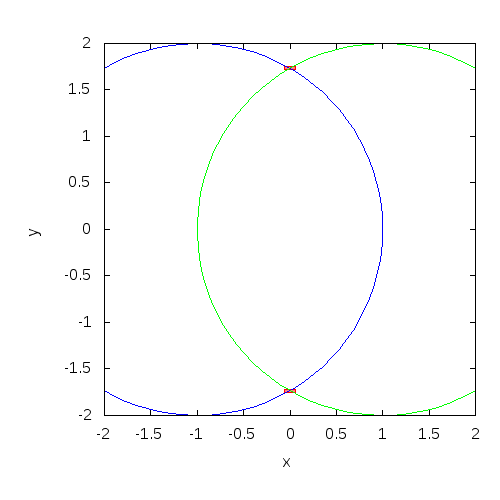
\includegraphics[scale=0.55]{img/circle-circle}
  %~ \caption{Intersection de deux cercles} %la légende
 %~ \label{fig:Deuxcerlces} %la légende	
%\end{figure} %on ferme l'environnement figure
On visualise ici que les solutions sont encadrées par des \og boîtes \fg{} rouges, et non réduites à des points. 

Dans le cas du problème \ref{eq2}, il serait possible d'avoir des solutions différentes selon la consistance choisie. Avec une hull-consistance, nous obtiendrions une boite contenant les deux solutions mais aussi une bonne partie de l'intersection des deux cercles. La \emph{3B-consistance} est une méthode plus puissante. Cette méthode vérifie, à l'instanciation de deux variables, vérifie localement toutes les contraintes. Une illustration des différences entre ces méthodes est proposée sur la figure \ref{fig:3Bconst}. Le problème résolu est celui de l'intersection de deux disques.
\begin{figure}[ht!] %on ouvre l'environnement figure
  \center
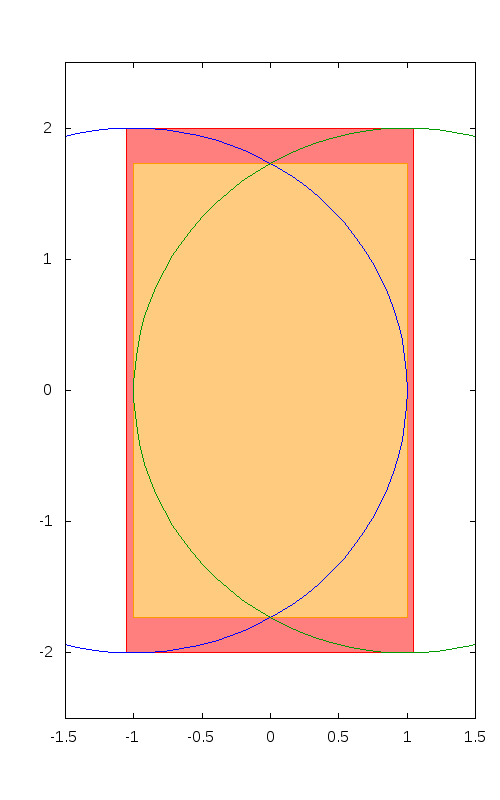
\includegraphics[scale=0.35]{img/disk-disk2}
  \caption{Comparaison graphique entre la Hull-consistance (rouge) et la 3B-consistance (orange)} %la légende
 \label{fig:3Bconst} %la légende	
\end{figure} %on ferme l'environnement figure


\subsection{Exemples d'application}

La précision de la méthode attirent le monde industriel. Notamment les applications composées de contraintes géométriques comme la robotique. La figure \ref{fig:rob} illustre un robot avec deux points d'encrage ($P_1$ et $P_2$) possédant chacun un bras rotatif de longueurs respectives [$L_1$] et [$L_2$] et orientés respectivement par les angles $\alpha_1$ et $\alpha_2$. Ces bras sont composés de pistons permettant d'ajuster leurs longueurs. Ainsi leurs longueurs de bras sont comprises respectivement entre $[L_{1min} \dots L_{1max}]$ et $[L_{2min} \dots L_{2max}]$ et les angles entre $[\alpha_{1min} \dots \alpha_{1max}]$ et $[\alpha_{2min} \dots \alpha_{2max}]$.  

\begin{figure}[h] %on ouvre l'environnement figure
  \center
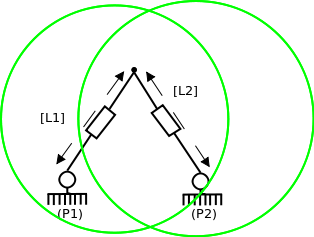
\includegraphics[scale=0.80]{img/robot2}
  \caption{Exemples d'application dans la robotique} %la légende
 \label{fig:rob} %la légende
\end{figure} %on ferme l'environnement figure
L'objectif est de connaître l'ensemble des emplacements possibles pour la main du robots en fonction des paramètres donnés ci-dessus. Dans le cas de la figure \ref{fig:rob}, on peut considérer que les $L_{imin}$ sont nulles et que les bras puissent effectuer des rotations de $360 \degres$. Ainsi le problème consiste à retrouver l'intersection de deux disques. 

  Par ailleurs, ces méthodes intéressent régulièrement les industriels. On retrouve en effet dans \cite{Schichl}, les détails d'applications dans le secteur de la chimie industrielle mais aussi dans celui de la biologie avec une étude sur les protéines. La science fondamentale met aussi en application ces outils. C'est le cas en mathématique par exemple de problèmes tel que la conjecture de \textsc{Kepler} ou encore le  maximum de clique.

\clearpage

\section{Mise en œuvre de la méthode de résolution par intervalles}



\subsection{Algorithmes}
L'algorithme de \emph{Branch and Prune} est au centre de la méthode de résolution par intervalles. Nous résumons ici ses deux étapes :  % met en oeuvre deux opérations détaillées dans \cite{Neumaier}: \\
%\begin{itemize}
%\item{Branch}
\paragraph{Branch :}
\begin{quote}\emph{Diviser pour mieux régner}\end{quote} Cette méthode consiste à diviser récursivement un problème en deux sous problèmes. Appliquée à la méthode de résolution par intervalles, on découpe en deux l'intervalle concerné (en son milieu ou non). On obtient alors deux problèmes plus \og petits \fg{} à étudier.%\clearpage
%\item{Prune}\\

\paragraph{Prune :}
La découpe d'un problème en sous problèmes peut amener à une situation ou un des sous problèmes créés ne contient aucune solution. On peut alors étudier et trier ces sous problèmes pour en supprimer les espaces de recherche superflus. Cette étape est appelée \emph{pruning}.

Au bout d'un certain nombre d'itération, l'algorithme de \emph{Branch and Prune} propose un ensemble de solutions sous la forme d'intervalles.% On visualise sur la figure \ref{fig:CercleDisque} un tel ensemble dans le cas d'une intersection entre un cercle et d'un disque.





\subsection{Données en sortie}
En sortie l'algorithme va nous retourner un ensemble de boîtes. Cet ensemble garantissant, à contrario des méthodes numériques classiques, que toutes les solutions y sont incluses. Dans la section \ref{par:out} un exemple d'illustration d'un tel ensemble est donné.

%~ \begin{figure}[h!] %on ouvre l'environnement figure
  %~ \center
%~ 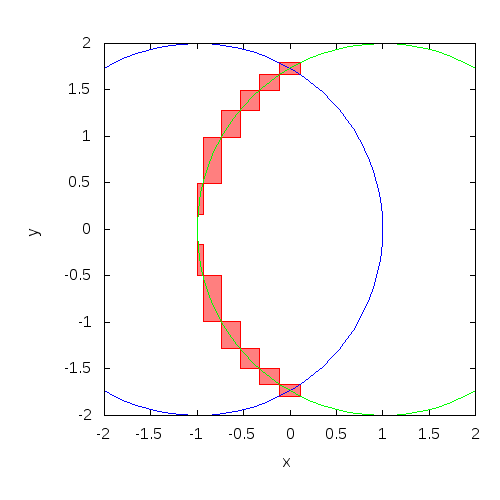
\includegraphics[scale=0.5]{img/circle-disk}
  %~ \caption{Intersection d'un cercle et d'un disque} %la légende
 %~ \label{fig:CercleDisque} %la légende
%~ \end{figure} %on ferme l'environnement figure

 Il est d'ailleurs possible de savoir si tout l'espace d'une boîte est solution du problème. En contrepartie on ne peut toujours garantir l'existence d'une solution dans une enveloppe, il peut donc exister une approximation autour des résultats de l'algorithme.

\clearpage
 
 \section{Applications par des outils}
\subsection{Realpaver}\label{realp}
Développé  au sein de l'équipe \textsc{OPTI}, cet outil reprend, entre autres, les méthodes de résolutions de contraintes géométriques par propagation d'intervalles. Il permet la résolution de systèmes d'équations à $n$ variables représentant des contraintes. Dans un soucis de précision ces solutions sont sous la forme d'intervalles \cite{realpaver}.% Les figures présentées dans ce chapitre (\ref{fig:Deuxcerlces}, \ref{fig:3Bconst} et \ref{fig:CercleDisque}), correspondent à des pavages calculés par cet outil. \cite{realpaver}.
\paragraph{Problème}
Soient deux disques, l'un de centre $(-1,0)$ et l'autre de centre $(1,0)$. Tous deux sont de rayon $2$. Donnez l'ensemble des solutions de l'intersection de ces deux disques.
\paragraph{Modèle}
L'outil \realpaver{}  modélise un tel problème de la sorte :
\label{realprob}
\begin{verbatim} 
Constants
  x0 = -1,
  y0 = 0,
  R0 = 2,
  x1 = 1,
  y1 = 0,
  R1 = 2
;
Variables
  x in ]-oo, +oo[,
  y in ]-oo, +oo[
;
Constraints
  (x-x0)^2 + (y-y0)^2 <= R0^2,
  (x-x1)^2 + (y-y1)^2 <= R1^2
;
\end{verbatim}
\paragraph{Données en sortie}\label{par:out}
L'ensemble de solutions suivant \realpaver{} propose l'ensemble de solutions suivant : 

\begin{verbatim}
RealPaver v. 0.4 (c) LINA 2004

INITIAL BOX
  x in ]-oo , +oo[
  y in ]-oo , +oo[

OUTER BOX 1
  x in [0.7924334198270921 , 0.795689483022687]
  y in [0.8806243697296342 , 0.8872330220900007]

...

OUTER BOX 3053
  x in [-0.7956894830226868 , -0.7924334198270919]
  y in [-0.8872330220900011 , -0.8806243697296345]

  precision: 0.00661, elapsed time: 150 ms

END OF SOLVING
  Property:     reliable process (no solution is lost)
  Elapsed time: 150 ms
\end{verbatim}
Ces 3053 solutions proposées par \realpaver{} sont illustrées sur la figure \ref{fig:DisqueDisque}.
\begin{figure}[ht!] %on ouvre l'environnement figure
  \center
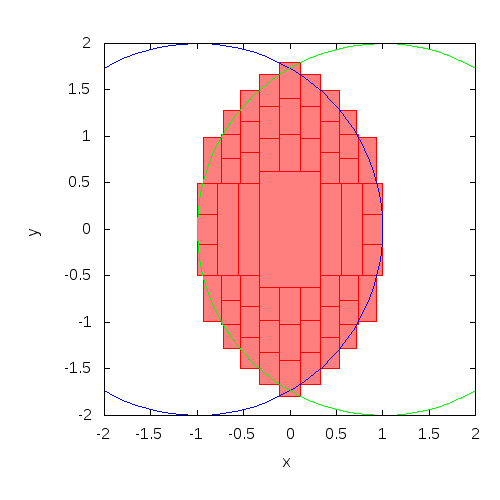
\includegraphics[scale=0.40]{img/disk-disk}
  \caption{Intersection de deux disques} %la légende
 \label{fig:DisqueDisque} %la légende
\end{figure} %on ferme l'environnement figure
\clearpage
\subsection{Autres outils existants}
\begin{description}
\item [CHOCO]  Projet commun  de l'École des Mines de Nantes, de \textsc{LIRMM} de Montpellier ansi que l'\textsc{INRA} de Toulouse. \textsc{CHOCO} est une librairie  \textsc{JAVA}  dédiée au résolution de \textsc{CSP} et à la programmation par contrainte. \cite{choco}
 \begin{figure}[h] %on ouvre l'environnement figure
  \center

\includegraphics[scale=0.50]{img/choco}
\end{figure} %on ferme l'environnement figure
\item [Google or-tools]
 Bibliothèque Python fournissant un solveur de contraintes générique et divers algorithmes, notamment sur les problèmes de graphes ou de sacs à dos : \cite{ortools}


\end{description}


\chapter{Contributions}\label{chap:con}


%nombre de caractéristiques ?? de quels type 

%Regarder JDK allocation d'une boite structure


%lister toutes les possibilité - garder toutes les structures - reconstruire l'arbre.. refaire une passe sur le fichier


\section{Introduction}
Trois difficultés majeures apparaissent dans la réalisation du logiciel de visualisation. La première est bien entendu la gestion d'une très grande quantité de boîtes lors de l'affichage. Il est en effet nécessaire d'offrir un accès rapide aux informations des boîtes dans la fenêtre. La seconde est la gestion des filtres sur ces mêmes boîtes. Et le troisième apparait lors du changement des variables étudiées (changement des dimensions visualisées). Dans cette section, nous chercherons d'avantage à apporter une solution pour les problèmes de temps d'accès et de changement de variables. Il est en effet probable que la gestion des filtres soit effectuée par une structure différente.
\\ \\

L'objectif de ce document est de mener une étude sur les différentes structures de données nécessaires aux futurs algorithmes de visualisation. Nous nous intéresserons en particulier à l'opération d'accès à une caractéristique ou d'une donnée d'une boîte ainsi qu'à l'occupation mémoire de cette dernière. Il s'appuie sur le document de spécification (cf. \ref{sec:spe}). Ce document sur les calculs de complexité seront réalisés selon le paramètre $n$  représentant le nombre de boîtes, et $d$ est le nombre de dimensions du problème. Le nombre de boîtes réellement utilisées dans le pavage est représenté par $N$. 


\section{Définition de la boîte}
C'est l'entité atomique du pavage. Les accès à ses attributs sont donc cruciaux. On rappelle qu'une boîte est définie de la manière suivante : 
\begin{itemize}
\item 
  Un identifiant : soit des chaînes de caractères (IDStr) respectant un format précis (cf. 1.1 du document de spécifications), soit des entiers positifs (IDInt).
\item
  Une liste de coordonnées dans l'ordre des variables définies en entête. Une liste de type \verb+Interval+.
\item
  Une liste des caractéristiques, dans l'ordre et selon les types définis en entête.
\end{itemize}
Ces données seront régulièrement requises lors de la mise en œuvre des algorithmes nécessaires à la visualisation. Il est donc important que leurs accès soient rapides, voire directs. Pour le cas de l'identifiant, s'agissant d'une simple \verb+String+ le problème de la structure à utiliser ne se pose pas. Pour la liste des coordonnées en revanche, il s'agit d'une séquence finie de données. Plusieurs possibilités sont alors envisageables : 

\begin{itemize}
\item
  Un tableau : L'accès à une coordonnée est direct. Les opérations d'ajout et de suppression sont en revanches coûteuses pour les tableaux dynamiques ($O(n)$).
\item
  Une liste : Si l'accès à une coordonnée n'est pas direct ($O(n)$), les opérations d'ajout et de suppression sont en temps constant.
\item
  Une table de hachage : Coûteuse si la fonction de hachage n'est pas appropriée, une table de hachage propose cependant un accès en $O(1)$.  Cependant le phénomène de collisions (mauvaise répartition des clefs entrainant un conflit entre deux valeurs) est à prendre en considération :

\begin{description}
\item[Implémentation avec un tableau dynamique] Une telle structure permet de garantir un accès en temps constant. Cependant chaque collision va doubler l'occupation mémoire du tableau. Or même si la fonction de hachage est bonne, il est possible d'avoir au moins une collision, ce qui aurait pour conséquence une perte de l'espace mémoire qui se répercuterait sur chaque boîte.
\item[Gestion des collisions avec chaînage] Contrairement à la structure précédente, cette méthode permet de ne pas occuper trop d'espace en chainant les éléments entrants en collision. Malheureusement la complexité en pire cas des opérations d'accès passe en $O(n)$. En revanche, grâce à une bonne fonction de hachage, on accèdera généralement en temps constant sans contre coût mémoire. 
\end{description}

Le passage en revue de ces différentes structures écarte la liste et la table de hachage implémentée par un tableau dynamique. En effet les performances des opérations d'accès de la liste ne sont pas raisonnables. De même l'implémentation d'une table de hachage par un tableau dynamique risque d'entrainer une perte de mémoire trop importante.
%\item
 % Une TreeMap \cite{TreeMap}. Implémentation de base des arbres rouges noirs, cette map a la particularité de posséder des clefs triées. Ainsi les complexités de plusieurs opérations telle que l'accès en $O(\log{n})$. Dans le cas d'un grand nombre de valeurs à stocker, il est plus performant de construire la TreeMap à partir d'une HashMap.

\end{itemize}

%La création d'une boîte a alors une complexité en $O(d)$. De plus l'accès aux différents attributs de la boîte (identifiant, liste des coordonnées) sera en $O(1)$.

\subsection{Généricité des caractéristiques}
Un problème majeur apparaît pour l'instanciation des boîtes. On rappelle qu'une caractéristique à plusieurs types (\verb+String+, \verb+Number+ ou \verb+Interval+). Plusieurs solutions sont envisageables : 
\begin{itemize}
\item
  Une Map unique contenant des \verb+String+ stocke les différentes caractéristiques de la boîte. On aura casté les attributs \verb+Number+ ou \verb+Interval+ en \verb+String+. Il sera alors nécessaire, pour chaque futurs accès, d'effectuer un cast dynamique. On rajoute alors une constante supplémentaire à la complexité de cette opération. 
\item 
Trois tableaux (un pour chaque type) au sein d'une boîte. Trois Maps (une pour chaque type) «générales» au niveau du pavage. La clef d'une map est l'id de la caractéristique et la valeur de la map son indice dans le tableau concret. La boîte peut alors retrouver la valeur de la caractéristique au sein de son tableau.
\item 
  Chaque boîte possède trois Maps pour ces trois types de caractéristiques. 
\end{itemize}


\section{Pavage}
\subsection{Problématique}
%L'outil de visualisation peut charger un fichier entrée de manière dynamique ou non. Nous nous plaçons ici dans le cadre où cette option de chargement dynamique n'est pas activée. \\ 
%L'outil va lire séquentiellement chaque ligne du fichier d'entrée.
Le cahier de spécification exige de l'outil la capacité à charger un pavage de taille non déterminée. Si le nombre de boîtes sera en pratique nécessairement borné (limite mémoire de la machine), il faut cependant répondre à cette attente en proposant une structure de stockage capable de supporter un très grand nombre de boîtes. De plus l'outil doit être en mesure de fournir régulièrement des listing spécifiques de boîtes. Par exemple pour afficher la liste de celles concernées par un \emph{filtre} (cf. \ref{sec:spe} section 1.2, 5\up{ème} point). La structure du pavage doit être en mesure de répondre de manière efficace à des requêtes de séquences de boîtes selon un ordre particulier. La structure du pavage doit être aussi en mesure de répondre efficacement à la structure  de visualisation graphique (fournir rapidement les nouvelles boîtes dans le champs de visualisation, lors d'une rotation de caméra par exemple). Quelles structures de données et quelles stratégies choisir face à de telles exigences ?  %Ce chapitre débute par de le passage en revue de différentes structures de données potentielles. % La création de la structure de stockage débute par la lecture séquentielle du fichier d'entrée (cf section 1  du document de spécification). Plusieurs options apparaissent à cette étape, faut-il par exemple :



\subsection{\'Etude de structures}

\paragraph{Vector :} Collection de données à accès direct par indice. Le nombre de boîte étant donné dans l'entête du fichier d'entrée, une implémentation par un tableau statique proposerait une complexité en temps et en espace égale à $O(n)$ pour l'opération de stockage du pavage. Si l'accès à une boîte à partir de son indice serait direct, l'opération de recherche en revanche aurait une complexité en temps égale à $O(n)$. 

\paragraph{Dictionnaire :} Collection de données à accès direct par clef. Dans l'hypothèse de posséder une fonction de hachage ne provoquant pas de collisions, une implémentation par une fonction de hachage propose une complexité en temps et en espace égale à $O(n)$ (à nouveau grâce à la connaissance du nombre de boîtes dans l'entête du fichier d'entrée).


%Le nombre potentiellement très grand de boîtes élimine d'emblée la possibilité de choisir une HashMap. En effet même si la fonction de hashage est judicieusement choisie, l'occupation mémoire requise serait bien trop importante. Les listes ne sont pas  appropriées ici. Une complexité en $O(n²)$ pour un accès à une boîte n'est pas raisonnable. Les arbres ont l'atout de pouvoir stocker et manipuler un grand nombre de d'entités. Les arbres de recherches sont des arborescences ordonnées permettant un accès en $O(\log(n))$. Dans le cas où la structure serait triée au fur et à mesure de sa construction. Les arbres de recherche proposent de bonnes performances. Nous développerons pourquoi à travers des cas d'exemples dans les prochains paragraphes : 

\clearpage
\paragraph{Arbre binaire}
L'utilisation d'un arbre binaire de recherche pour la création de $n$ boîtes aurait une complexité en espace et en temps égale à $O(n²)$ en pire cas. En effet il s'agit du cas où les boîtes arriveraient triées selon l'ordre inverse de celui que l'on souhaite. Ce critère d'ordonnancement des boîtes peut varier (Id, caractéristique «temps de calcul», borne inférieur d'une variable, \dots{}). Il faudrait alors effectuer $(p-1)$ comparaisons, pour chaque boîte :  $\sum_{p=2}^{n}(p-1)$  Soit une compléxité en temps égale à $O(n)=\frac{1}{2}n²-\frac{1}{2}n$. Cependant dans le meilleur des cas, cette opération a une complexité en $O(n\log{n})$. La création d'un pavage composé de $n$ boîtes à $d$ dimensions aurait alors une complexité en temps égale à: $O(d \times n\log(n))$.

\begin{figure}[htbp]
  \centering
  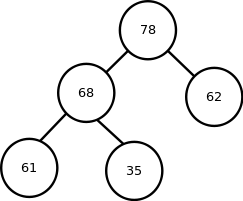
\includegraphics[scale=0.60]{img/binTree}
  \caption{arbre binaire}
  \label{fig:abtree}
\end{figure}
L'arbre binaire était équilibré par définition, la complexité de son opération de recherche est en $O(log_2 n)$ (hauteur de l'arbre).
   


%http://www.enseignement.polytechnique.fr/profs/informatique/Luc.Maranget/421/poly/arbre-bin.html
%\clearpage
\paragraph{Arbres a-b}
Il s'agit d'un arbre de recherche avec les propriétés suivantes :
\begin{itemize}
\item
  $a\leq2$ et $b\leq 2a−1$ deux entiers.
\item
  La racine a au moins 2 fils (sauf si l'arbre ne possède qu'un nœud) et au plus b fils.
  Les feuilles sont de même profondeur.
\item
  Les autres nœuds internes ont au moins a et au plus b fils.
\end{itemize}

\begin{figure}[h!tbp]
  \centering
  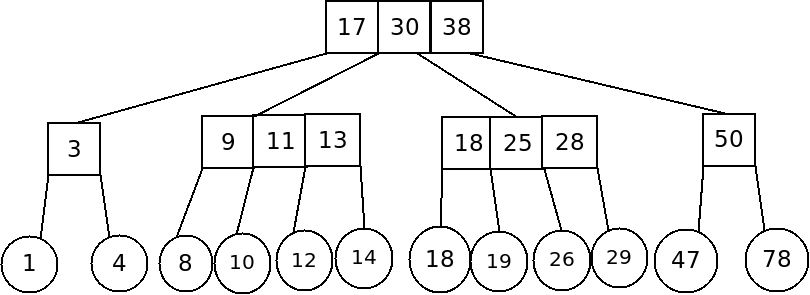
\includegraphics[scale=0.40]{img/abtree}
  \caption{a-b arbre}
  \label{fig:abtree}
\end{figure}

L'avantage des arbres a-b est que leurs hauteurs  sont comprises entres les valeurs suivantes : $ \dfrac{\log{n}}{\log{b}}   \leq h  < 1 + \dfrac{\log{n/2}}{\log{a}}$. Ainsi les opérations d'insertion ne seraient plus en $O(n\log{n})$ mais en $O(\log{n})$. La création d'un pavage composé de $n$ boîtes à $d$ dimensions aurait alors une complexité en $O((n\times d)\log(n))$. La recherche d'un boîte quant à elle aurait une complexité en $O(\log{n})$.

{\color{red}* à la fin de la section 1, il manque une discussion sur les différentes 
possibilités passées en revue assortie d'une recommandation pour tel ou 
tel usage. Vous devriez aussi y mentionner que plusieurs structures 
pourraient être maintenues parallèlement pour offrir un accès facilité 
pour telle ou telle opération importante (vue, filtre, ...) mais mettre 
en garde concernant le maintient de cohérence de ces structures et le 
coût mémoire de cette redondance.
}
\section{Stockage des boîtes et visualisation}

\subsection{\'Etude d'une solution possible : le QuadTree}
\paragraph{}Une des solutions qui pourrait permettre une visualisation fluide du pavage tout en répondant au document de spécifications serait de représenter le pavages sous une forme de QuadTree pour deux dimensions ou OcTree pour trois dimensions.
\begin{figure}[htbp]
\centering
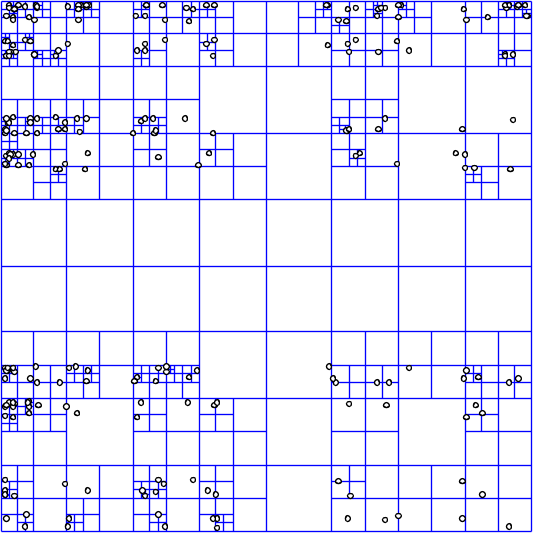
\includegraphics[scale=0.50]{img/quadtree}
\caption{Représentation d'un QuadTree où les données sont des points}

\end{figure}

Le QuadTree consiste à découper récursivement un espace fini en deux dimensions en quatre parties égales. Chacune de ces parties sont stockées dans un nœud. On itère ce mécanisme sur chacun de ces nœuds jusqu'à isoler spatialement les éléments recherchés.

Cette structure pourrait être utilisée pour déterminer la position des boîtes dans l'espace.

\paragraph{}L'algorithme permettant de partitionner est récursif. Dans le cas récursif, l'algorithme divise l'espace en quatre et itère sur chaque sous-espace. Dans le cas d'arrêt on ne subdivise plus. Nous décrivons par la suite l'ensemble des cas de récursions et d'arrêts pour la division d'un espace donné. Les images jointes au texte sont des représentations des différents cas dans lesquels les cadres rouges sont des boîtes solutions et les cadres noirs un espace fourni à l'algorithme. Vous trouverez une classification visuelle dans la table \ref{tab:algo}.
\begin{itemize}
\item Cas d'arrêts : 
\begin{itemize}
\item L'espace fourni est entièrement inclus dans une boîte 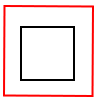
\includegraphics[scale=0.20]{img/QT1}.
\item L'espace fourni contient entièrement une seule boîte 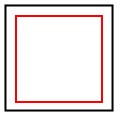
\includegraphics[scale=0.20]{img/QT2}.
\item L'espace fourni contient en partie une seule boîte 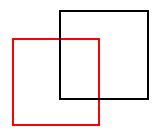
\includegraphics[scale=0.20]{img/QT3}.
\item L'espace fourni n'intersecte aucune boîte 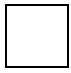
\includegraphics[scale=0.30]{img/QT6}.
\item L'espace fourni ne peux plus être subdivisé car on a fourni une taille minimale pour les espaces.
\end{itemize}
\item cas de récursions :
\begin{itemize}
\item L'espace fourni intersecte plusieurs boîtes 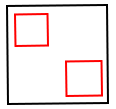
\includegraphics[scale=0.20]{img/QT4} ou encore 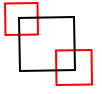
\includegraphics[scale=0.20]{img/QT5}.
\end{itemize}
\end{itemize}

\begin{table}[htbp]
\centering
 \begin{tabular}{|c|cccc|}
  \hline
  Cas de récursion &  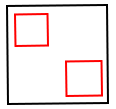
\includegraphics[scale=0.20]{img/QT4}&  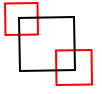
\includegraphics[scale=0.20]{img/QT5}& &\\
  \hline
  Cas d'arrêt&  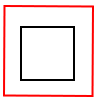
\includegraphics[scale=0.20]{img/QT1}&  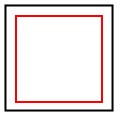
\includegraphics[scale=0.20]{img/QT2}&  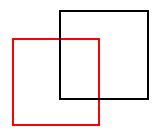
\includegraphics[scale=0.20]{img/QT3}&  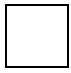
\includegraphics[scale=0.30]{img/QT6}\\
  \hline
 \end{tabular}
 \caption{Classification visuelle des cas d'arrêts et de récursions}
\label{tab:algo}
\end{table}


L'OcTree repose sur le même principe mais étendu à trois dimensions. L'espace est donc découpé en huit parties à chaque fois.

\paragraph{Avantage de cette méthode}Cette structure est particulièrement intéressante pour la visualisation du pavage. En effet pour une fenêtre de visualisation donnée, il est très simple et rapide d'extraire la sous-arborescence correspondante à l'espace visualisé et permet aussi de ne pas afficher les objets trop petits. 

De plus il serait possible de créer une structure reposant sur le même principe que le QuadTree mais étant $k$-dimensionnelle\footnote{$k$ étant la dimension du problème fourni à RealPaver.}. Chaque espace peut alors être potentiellement subdivisé en $2^k$ sous-espaces. Cette structure permettrait d'éviter de recalculer l'arbre à chaque changement de variables de visualisation. On évite par ailleurs le cas de superposition de boîtes pour lequel l'algorithme n'est plus efficace (cf : figure \ref{fig:superpos}).
\begin{figure}[htbp]
\centering
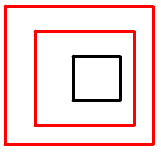
\includegraphics[scale=0.30]{img/QT8}
\caption{Superposition de boîtes}
\label{fig:superpos}
\end{figure}

\paragraph{Inconvénient de cette méthode}Le problème majeur de cette méthode se présente lorsque des boîtes sont côte à côte (cf : figure \ref{fig:frontiere}).
\begin{figure}[htbp]
\centering
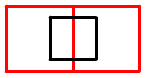
\includegraphics[scale=0.40]{img/QT7}
\caption{Superposition de boîtes 1}
\label{fig:frontiere}
\end{figure}
Dans une telle situation chaque division va entrainé la création d'un espace dans la même configuration. L'algorithme ne s'arrêtera donc pas avant d'avoir atteint la taille minimale d'un espace. Nous nous retrouvons donc avec un grand nombre de boîtes au niveau de ces \og frontières\fg{} (cf : figure \ref{fig:frontiere2}).
\begin{figure}[htbp]
\centering
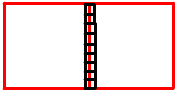
\includegraphics[scale=0.40]{img/QT9}
\caption{Superposition de boîtes 2}
\label{fig:frontiere2}
\end{figure}
Ainsi sachant que la précision maximale par défaut de \emph{RealPaver} est de $10^{-16}$, cela implique qu'il est nécessaire d'au moins égaler cette précision pour l'arbre de visualisation. Ainsi pour une sortie de \emph{RealPaver} contenant un total $l$ de longueurs de \og frontières \fg{}  cumulées et $p$ la précision du modèle, on a un nombre d'espaces à créer supérieur à $\frac{l}{p}$ avec $p$ très petit. Par exemple pour une sortie de \emph{RealPaver} comportant une \og frontière \fg{} de taille $1$, il faudra au moins $10^{16}$ espaces pour la contenir. 

\paragraph{Brève conclusion} Le QuadTree est une structure intéressante pour la visualisation mais si un nœud de l'arbre a un coût en mémoire non nul, alors l'espace mémoire de la structure va exploser. Elle semble donc, pour le moment, inappropriée.

\section{\'Etude d'une seconde solution : le R-tree}
\paragraph{}Bien que le QuadTree soit une structure intéressante pour permettre l'indexation et la recherche de points dans un espace, celui-ci l'est beaucoup moins pour la gestion de données à dimensions non nulles. Le R-tree est une structure proposé en 1984 par Antonin \textsc{Guttman} permettant l'indexation et la recherche d'éléments de dimension $d > 0$ dans $k$ dimensions\cite{Guttman}.

\paragraph{}Le R-tree est une variante équilibré de l'arbre B, sa structure est la suivante :
\begin{itemize}
 \item Un noeud de l'arbre correspond à une boîte non-solution du pavage ( généralement appelé \og page \fg{}).
 \item Chaque boîte peut contenir entre $m$ et $M$ sous-boîtes entièrement incluses. Avec $m\leq \frac{M}{2}$.
 \item Une feuille de l'arbre est une boîte ne contenant que des boîtes solution du pavage.
\end{itemize}

La figure \ref{fig:rtree} donne une bonne idée de l'organisation des R-trees:
\begin{figure}[htbp]
\centering
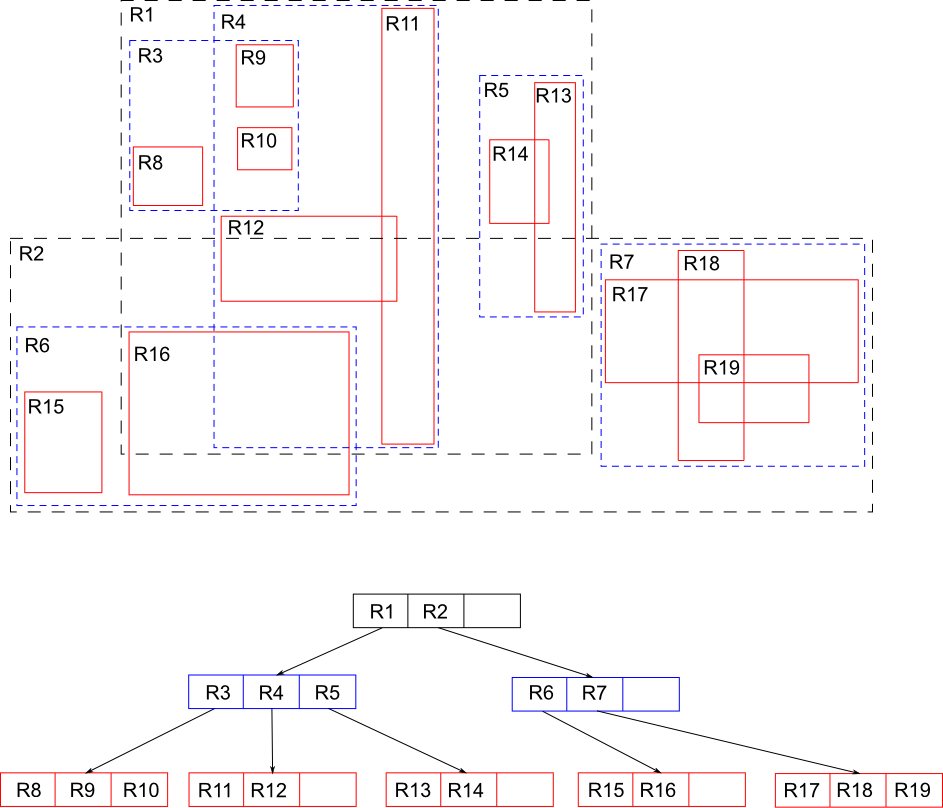
\includegraphics[scale=0.50]{img/rtree}
\caption{Représentation d'un R-tree\cite{wiki}}
\label{fig:rtree}
\end{figure}

Les algorithmes permettant la recherche et la création du R-tree sont qu'en à eux décrient dans l'article de \textsc{A. Guttman} dans la section \textbf{3. Searching and Updating}\cite{Guttman}.

\paragraph{Avantages et inconvénients du R-tree} Le R-tree est une structure de données spécialement conçue pour la recherche de données à dimensions $d$ pour dans des espaces $k$-dimensionnels. L'arbre a une profondeur maximale $h_{max}$ égale à :
\begin{equation}
 h_{max} = \left\lceil\log_{m} n\right\rceil - 1
\end{equation}
et le nombre de nœuds est au pire égale à :
\begin{equation}
 \sum_{i=1}^{h_{max}}{\left\lceil\frac{n}{m^i}\right\rceil} = \left\lceil\frac{n}{m}\right\rceil + \left\lceil\frac{n}{m^2}\right\rceil + \cdots + 1
\end{equation}

 Bien que ne pouvant garantir de bonnes performances en pire cas\footnote{\og \emph{More than one substree under a node may need to be searched, hence it is not possible to guarantee good worst-case performance.}\fg{}\cite{Guttman}, section \textbf{3.1 Searching}}, le R-tree offre en pratique de bons résultats ; on pourra d'ailleurs se reporter à l'analyse de performances effectuer par A. \textsc{Guttman}\footnote{section \textbf{4. Performance}\cite{Guttman}}. Cependant il existe aujourd'hui de nombreuses variantes du R-tree ( R*tree, Hilbert R-tree, etc\dots{} ), on pourra donc, pour une analyse plus générale des différentes implémentations, préférer \og\emph{R-trees : Theory and Applications} \fg{}\cite{poulos}.



\chapter{Étude pratique}
\section{Chargement de pavages}
\label{chap:Chargement}
Pour la génération des boîtes le nombre de caractéristiques est fixé à 20 et la dimension du pavage à 100. Ces valeurs ont été choisies car elles peuvent être considérées comme les valeurs au pire renvoyées par \realpaver. Cependant les caractéristiques pouvant être de différents types et ne connaissant pas la probabilité d'apparition de chacun de ces types, nous avons préféré construire des caractéristiques, générées aléatoirement, de chaque type en proportion un tiers (sept Number, sept String, six Interval). 

Tous les résultats sont répertoriés dans la partie \ref{sec:creation}.

\subsection{Map internes}

\subsubsection{Pavage avec une première proposition de structure}
Pour les Maps l'organisation des structures de données est la suivante :
\begin{itemize}
\item Il n'y a aucune structure de données globale, tout est stocké au niveau de la boîte. On a donc dans chaque boîte l'identifiant et la valeur de chaque caractéristique ou intervalle.
 \item Chaque boîte contient quatre Maps contenant les différentes informations :
\begin{itemize}
 \item Une Map pour l'ensemble des intervalles coordonnées.
\item Une Map pour les caractéristiques de type String.
\item Une Map pour les caractéristiques de type Interval.
\item Une Map pour les caractéristiques de type Number.
\end{itemize}
\end{itemize}

\paragraph{}Les résultats obtenus sont indiqués dans la table \ref{tab:hashmap1} et \ref{tab:treemap1}
D'après les résultats, les deux structures fournissent un temps de construction et une occupation mémoire similaires.
Il est encore difficile de déterminer laquelle de la TreeMap ou de la HashMap est la plus pertinente, les différences apparaîtront sans doute plus nettement au moment des tests d'accès aux caractéristiques. 


\subsubsection{Pavage avec une seconde proposition de structure}
Pour les map, une autre organisation des structures de données possible est la suivante :
\begin{itemize}
\item Il y a une HashMap globale contenant le type de chaque caractéristique.
 \item Chaque boîte contient deux Maps contenant les différentes informations :
\begin{itemize}
 \item Une map pour l'ensemble des intervalles coordonnées.
\item Une liste pour l'ensemble des caractéristiques stockées dans la boîte sous la forme d'Objects.
\end{itemize}
\end{itemize}

\paragraph{}Les résultats obtenus sont indiqués dans la table \ref{tab:hashmap3} et \ref{tab:treemap2}
Nous n'observons pas de différence nette, par rapport à la première proposition, quant au temps de construction et de l'occupation mémoire. Cette structure nécessitant d'effectuer un cast à chaque accès, il est plus avantageux de conserver la première structure.


\subsection{Listes et Tableaux internes}
Pour les structures liste et tableau l'organisation des structures de données est la suivante :
\begin{itemize}
\item Il y a une HashMap globale contenant le type de chaque caractéristique.
 \item Chaque boîte contient deux listes (ou tableaux) :
\begin{itemize}
 \item Une liste pour l'ensemble des intervalles coordonnées.
\item Une liste pour l'ensemble des caractéristiques de la boîte stockées sous la forme d'Objects
\end{itemize}
\end{itemize}

\paragraph{}Les résultats obtenus sont indiqués dans la table \ref{tab:arraylist} et \ref{tab:linkedlist}
On peut constater que les structures de données en liste sont bien meilleures vis-à-vis du temps de construction et de l'espace mémoire(Tout du moins pour l'ArrayList) que les structures map de la première partie. Étrangement la structure LinkedList demande un espace mémoire presque 60\% plus grand que celui alloué pour l'ArrayList.


\subsection{Maps globales}
Les boîtes sont composées  de 4 ArrayLists : 
\begin{itemize}
  \item Une ArrayList pour l'ensemble des intervalles coordonnées.
  \item Une ArrayList pour les caractéristiques de type String.
  \item Une ArrayList pour les caractéristiques de type Interval.
  \item Une ArrayList pour les caractéristiques de type Number.
\end{itemize}
Il faut cependant savoir à quels indices se trouves les différents élément pour effectuer des accès directs. Pour cela, on dispose ici de quatre Maps globales :
\begin{itemize}
  \item Une Map pour l'ensemble des intervalles coordonnées.
  \item Une Map pour les caractéristiques de type String
  \item Une Map pour les caractéristiques de type Interval
  \item Une Map pour les caractéristiques de type Number
\end{itemize}
La composition de chacune de ces maps est la suivante :  
\begin{description}
 \item[Clef :]
ID de la coordonnée ou de la variable.
\item[Valeur :]
Indice de l'objet dans le tableau de la boîte.
\end{description}


\paragraph{Observations :}
On propose trois cas de tests ou les Maps globales seront :
\begin{itemize}
  \item Des HashMaps :  \ref{tab:hashmapglobal} 
  \item Des TreeMaps :  \ref{tab:treemapglobal} 
\end{itemize}
Les trois cas de tests nous renvoient des résultats relativement similaires mais qui se montrent aussi performants que les résultats de l'ArrayList. Il s'agit donc d'une organisation intéressante à étudier au niveau des temps d'accès.




\section{Accès aux éléments d'une boîte}
Dans cette partie nous allons effectuer des tests d'accès aux éléments d'une boîte. Le nombre de coordonnées et de caractéristiques sont les mêmes que dans la partie \ref{chap:Chargement} c'est-à-dire 100 valeurs pour les coordonnées et 20 caractéristiques. Parmi ces coordonnées, sept sont de type \verb+Number+, sept de type \verb+String+ et 6 de type \verb+Interval+. Pour toutes les structures testées, il est nécessaire d'avoir une structure globale contenant les types de chaque caractéristique. Nous effectuerons d'abord des tests d'accès au caractéristiques puis des tests d'accès au coordonnées. Nous rappelons aussi que les éléments sont générés aléatoirement durant la création.

Pour plus d'aisance, nous considérerons que les identifiants sont de types \verb+Integer+. Un type \verb+String+ revenant au final au même mais nécessitant au préalable un hashage.

Il est aussi important de préciser que, pour tester, nous avons créé dix-mille boîtes et que pour accéder à une caractéristique, nous accédons d'abord à une boîte aléatoirement. Les boîtes sont stockées dans un tableau de taille statique à accès direct par indice. Même s'il est vrai que cette méthode introduit une constante dans le calcul de la complexité, elle permet de ne pas toujours accéder à la même information et donc de ne pas permettre un accès plus rapide qui ne serait pas réaliste.

Tous les résultats sont répertoriés dans la partie \ref{sec:acces}.

\subsection{Tests d'accès aux caractéristiques}
Pour les tests d'accès aux caractéristiques, nous générons aléatoirement un nombre donnant l'identifiant de la caractéristique.

\paragraph{} Les résultats d'accès pour des boîtes contenant une Map (HashMap ou TreeMap) par type de caractéristique (\verb+Number+, \verb+String+ ou \verb+Interval+) sont indiqués dans le tableau \ref{tab:accesHM}.

On peut voir que les deux structures ne se distinguent pas beaucoup en terme de performance, on observe seulement un écart de moins d'une seconde entre la HashMap et la TreeMap à partir de cent millions d'accès.


\paragraph{} Les résultats d'accès pour des boîtes contenant une Map (HashMap ou TreeMap) pour stocker toutes les caractéristiques sont indiqués dans le tableau \ref{tab:accesHM2}.

Cette fois ci les résultats sont légèrement différents pour les deux structures. La HashMap est en effet plus efficace que le TreeMap de presque 10\%, elle est d'ailleurs plus efficace que lorsque chaque caractéristique était stockée dans sa propre Map.

\paragraph{} Les résultats d'accès pour des boîtes contenant une ArrayList ou une LinkedList pour stocker toutes les caractéristiques sont indiqués dans le tableau \ref{tab:accesAL}.

On peut nettement voir l'efficacité de la structure ArrayList pour les temps d'accès par rapport à la LinkedList, mais aussi par rapport à toutes les autres structures précédemment proposées. Celle-ci étant plus efficace de 40\% à 50\% par rapport aux autres structures. On peut aussi s'étonner des performances de la LinkedList par rapport aux structures Maps, mais on peut supposer que leur proximité est due au faible nombre de caractéristiques à stocker.

\paragraph{} Les résultats d'accès pour des boîtes contenant une ArrayList pour chaque caractéristique, avec une Map globale pour retrouver les indices de chacune de ces caractéristiques dans les boîtes, sont indiqués dans le tableau \ref{tab:accesHMG}.

D'après les résultats, l'utilisation d'une HashMap globale est environ 10\% plus efficace que d'utiliser une TreeMap globale. La structure proposée avec une HashMap globale offre de bonnes performances par rapport aux autres structures proposées précédemment, mais reste tout de même moins efficace qu'une ArrayList stockant toutes les caractéristiques.

\paragraph{Conclusion sur l'accès aux caractéristiques} Les meilleures performances sont obtenues lorsqu'une boîte ne contient qu'une ArrayList pour stocker toutes les caractéristiques. Cependant on peut se demander s'il peut s'avérer utile d'obtenir uniquement les caractéristiques pour un type donné. Si c'est le cas, il sera nécessaire d'effectuer une recherche au préalable pour obtenir les éléments désirés. Tandis que lorsque les boîtes contiennent une ArrayList pour chaque caractéristique, bien que les performances d'accès unique soient légèrement moins bonnes, cette recherche serait alors inutile.

\subsection{Tests d'accès aux coordonnées}
 Les résultats d'accès aux coordonnées pour différentes structures (Map et List) sont détaillés dans le tableau \ref{tab:accesCoord}.

Sans surprise l'ArrayList reste la structure la plus adaptée pour stocker les coordonnées.

\section{Conclusion}
Au vu des résultats sur les différentes architectures, celle proposant que chaque boîte ne contiennent qu'une ArrayList pour stocker toutes les caractéristiques est la plus efficace, que ce soit au niveau des temps d'accès qu'au niveau des temps de construction et d'espace mémoire. Cependant l'architecture où les boîtes contiennent une ArrayList pour chaque caractéristique offre des résultats moins bons mais relativement proches, et permet une meilleure performance pour l'accès aux éléments d'un même type. Il sera donc nécessaire de voir si une telle action est utile.

Pour le stockage des coordonnées, l'utilisation de l'ArrayList est préconisée, les résultats la dégageant nettement du lot. 


\section{Annexes}
\subsection{Études de performance de création d'une boîte}
\subsubsection{Études de performance avec des Maps}

\begin{table}[htpb]
  \centering
\begin{tabular}{|c|c|c|c|}
\hline
Nombre de boîtes & CPU & Mémoire totale & Mémoire utilisée\\
\hline
100 & 0.05s & 52Mo & 1Mo\\
\hline
1000 & 0.09s & 52Mo & 7Mo\\
\hline
10000 & 0.16s & 119Mo & 70Mo\\
\hline
100000 & 0.86s & 776Mo & 667Mo\\
\hline
1000000 & \multicolumn{3}{|c|}{Out of memory}\\
\hline
\end{tabular}
\caption{Étude de performances avec des HashMap}
\label{tab:hashmap1}
\end{table}

\begin{table}[htbp]
  \centering
\begin{tabular}{|c|c|c|c|}
\hline
Nombre de boîtes & CPU & Mémoire totale & Mémoire utilisée\\
\hline
100 & 0.06s & 52Mo & 1Mo\\
\hline
1000 & 0.07s & 52Mo & 6Mo\\
\hline
10000 & 0.16s & 138Mo & 64Mo\\
\hline
100000 & 0.84s & 776Mo & 635Mo\\
\hline
1000000 & \multicolumn{3}{|c|}{Out of memory}\\
\hline
\end{tabular}
\caption{Étude de performances avec des TreeMap}
\label{tab:treemap1}
\end{table}

%\begin{table}[htbp]
%  \centering
%\begin{tabular}{|c|c|c|c|c|}
%\hline
%Nombre de boîtes & Temps écoulé & CPU & Mémoire totale & Mémoire utilisée\\
%\hline
%100 & 0.02125s & 0.06s & 52Mo & 1Mo\\
%\hline
%1000 & 0.04448s & 0.07s & 52Mo & 7Mo\\
%\hline
%10000 & 0.38182s & 0.15s & 123Mo & 69Mo\\
%\hline
%100000 & 10.61614s & 0.81s & 776Mo & 667Mo\\
%\hline
%1000000 & \multicolumn{4}{|c|}{Out of memory}\\
%\hline
%\end{tabular}
%\caption{Étude de performances avec des HashMap avec initialisation}
%\label{tab:hashmap2}
%\end{table}

\begin{table}[htbp]
  \centering
\begin{tabular}{|c|c|c|c|}
\hline
Nombre de boîtes & CPU & Mémoire totale & Mémoire utilisée\\
\hline
100 & 0.06s & 52Mo & 1Mo\\
\hline
1000 & 0.08s & 52Mo & 7Mo\\
\hline
10000 & 0.13s & 118Mo & 69Mo\\
\hline
100000 & 0.84s & 776Mo & 655Mo\\
\hline
1000000 & \multicolumn{3}{|c|}{Out of memory}\\
\hline
\end{tabular}
\caption{Étude de performances avec des HashMap seconde structure}
\label{tab:hashmap3}
\end{table}



\begin{table}[htbp]
  \centering
\begin{tabular}{|c|c|c|c|}
\hline
Nombre de boîtes & CPU & Mémoire totale & Mémoire utilisée\\
\hline
100 & 0.07s & 52Mo & 1Mo\\
\hline
1000 & 0.08s & 52Mo & 6Mo\\
\hline
10000 & 0.15s & 138Mo & 64Mo\\
\hline
100000 & 0.88s & 776Mo & 633Mo\\
\hline
1000000 & \multicolumn{3}{|c|}{Out of memory}\\
\hline
\end{tabular}
\caption{Étude de performances avec des TreeMap seconde structure}
\label{tab:treemap2}
\end{table}

\subsubsection{Études de performance avec des Tableaux et des Listes}

\begin{table}[h]
  \centering
\begin{tabular}{|c|c|c|c|}
\hline
Nombre de boîtes & CPU & Mémoire totale & Mémoire utilisée\\
\hline
100 & 0.05s & 52Mo & <1Mo\\
\hline
1000 & 0.06s & 52Mo & 4Mo\\
\hline
10000 & 0.09s & 66Mo & 37Mo\\
\hline
100000 & 0.30s & 408Mo & 342Mo\\
\hline
1000000 & \multicolumn{3}{|c|}{Out of memory}\\
\hline
\end{tabular}
\caption{Étude de performances avec des ArrayList}
 \label{tab:arraylist}
\end{table}

\begin{table}[htbp]
  \centering
\begin{tabular}{|c|c|c|c|}
\hline
Nombre de boîtes & CPU & Mémoire totale & Mémoire utilisée\\
\hline
100 & 0.05s & 52Mo & 1Mo\\
\hline
1000 & 0.08s & 52Mo & 5Mo\\
\hline
10000 & 0.1s & 88Mo & 54Mo\\
\hline
100000 & 0.30s & 776Mo & 542Mo\\
\hline
1000000 & \multicolumn{3}{|c|}{Out of memory}\\
\hline
\end{tabular}
\caption{Étude de performances avec des LinkedList}
\label{tab:linkedlist}
\end{table}
\clearpage




\subsubsection{Études de performance avec des maps globales}
%hashmap
\begin{table}[h]
  \centering
\begin{tabular}{|c|c|c|c|}
\hline
Nombre de boîtes & CPU & Mémoire totale & Mémoire utilisée\\
\hline
100 & 0.05s & 52Mo & 0Mo\\
\hline
1000 & 0.07s & 52Mo & 4Mo\\
\hline
10000 & 0.1s & 66Mo & 38Mo\\
\hline
100000 & 0.34s & 424Mo & 351Mo\\
\hline
1000000 & \multicolumn{3}{|c|}{Out of memory}\\
\hline
\end{tabular}
\caption{Étude de performances avec des HashMap globales} 
\label{tab:hashmapglobal}
\end{table}


%\begin{table}[h]
%  \centering
%\begin{tabular}{|c|c|c|c|c|}
%\hline
%Nombre de boîtes & Temps écoulé & CPU & Mémoire totale & Mémoire utilisée\\
%\hline
%100 & 0.00237& 0.05s & 52Mo & 0Mo\\
%\hline
%1000 & 0.03380 & 0.07s & 52Mo & 3Mo\\
%\hline
%10000 & 0.19556 & 0.09s & 89mo & 32mo\\
%\hline
%100000 & 2.0883 & 0.25s & 480mo & 312mo\\
%\hline
%1000000 & \multicolumn{4}{|c|}{Out of memory}\\
%\hline
%\end{tabular}
%\caption{Étude de performances avec des HashMap globales avec initialisation}
%\label{tab:hashmapglobalInit}
%\end{table}









%TreeMap
\begin{table}[h]
  \centering
\begin{tabular}{|c|c|c|c|}
\hline
Nombre de boîtes & CPU & Mémoire totale & Mémoire utilisée\\
\hline
100 & 0.05s & 52Mo & 0Mo\\
\hline
1000 & 0.06s & 52Mo & 4Mo\\
\hline
10000 & 0.11s & 66Mo & 38Mo\\
\hline
100000 & 0.38s & 422Mo & 350Mo\\
\hline
1000000 & \multicolumn{3}{|c|}{Out of memory}\\
\hline
\end{tabular}
\caption{Étude de performances avec des TreeMaps globales} 
\label{tab:treemapglobal}
\end{table}

%\begin{table}[h]
%  \centering
%\begin{tabular}{|c|c|c|c|c|}
%\hline
%Nombre de boîtes & Temps écoulé & CPU & Mémoire totale & Mémoire utilisée\\
%\hline
%100 & 0.008355 & 0.05s & 52Mo & 7Mo\\
%\hline
%1000 & 0.03096 & 0.06s & 52Mo & 6Mo\\
%\hline
%10000 & 0.181671s & 0.13s & 89Mo & 32Mo\\
%\hline
%100000 & 2.130028 & 0.30s & 481Mo & 318Mo\\
%\hline
%1000000 & \multicolumn{4}{|c|}{Out of memory}\\
%\hline
%\end{tabular}
%\caption{Étude de performances avec des TreeMaps globales avec initialisation}
%\label{tab:treemapglobalInit}
%\end{table}



% %TreeMap a partir de Hashmap
% \begin{table}[h]
%   \centering
% \begin{tabular}{|c|c|c|c|}
% \hline
% Nombre de boîtes & CPU & Mémoire totale & Mémoire utilisée\\
% \hline
% 100 & 0.05s & 52Mo & 0Mo\\
% \hline
% 1000 & 0.06s & 52Mo & 4Mo\\
% \hline
% 10000 & 0.11s & 66Mo & 38Mo\\
% \hline
% 100000 & 0.39s & 420Mo & 350Mo\\
% \hline
% 1000000 & \multicolumn{3}{|c|}{Out of memory}\\
% \hline
% \end{tabular}
% \caption{Étude de performances avec des TreeMaps construites à partir de HashMaps globales} 
% \label{tab:treehashmapglobal}
% \end{table}

%\begin{table}[h]
%  \centering
%\begin{tabular}{|c|c|c|c|c|}
%\hline
%Nombre de boîtes & Temps écoulé & CPU & Mémoire totale & Mémoire utilisée\\
%\hline
%100 & 0.008646 & 0.05s & 52Mo & 0Mo\\
%\hline
%1000 & 0.0.04127 & 0.07s & 52Mo & 6Mo\\
%\hline
%10000 & 0.18813s & 0.10s & 89Mo & 32Mo\\
%\hline
%100000 & 2.12998599 & 0.29s & 482Mo & 317Mo\\
%\hline
%1000000 & \multicolumn{4}{|c|}{Out of memory}\\
%\hline
%\end{tabular}
%\caption{Étude de performances avec des TreeMaps construites à partir de HashMaps globales avec initialisation} 
%\label{tab:treehashmapglobalInit}
%\end{table}

\subsection{Études de performance d'accès aux éléments d'une boîte}
\subsubsection{Comparaison des performances d'accès aux caractéristiques}
%Accès HashMap et TreeMap
\begin{table}[h]
  \centering
\begin{tabular}{|c|c|c|c|}
\hline
\backslashbox{Structure} {Nombre d'accès} & $10^6$ & $10^7$ & $10^8$ \\
\hline
HashMap & 0.31s& 2.86s & 28.56s\\
\hline
TreeMap & 0.30s & 2.82s & 27.84s \\
\hline
\end{tabular}
\caption{Relevé des temps CPU d'accès au caractéristiques en secondes pour la HashMap et la TreeMap} 
\label{tab:accesHM}
\end{table}

%Accès HashMap et TreeMap Unique
\begin{table}[h]
  \centering
\begin{tabular}{|c|c|c|c|}
\hline
\backslashbox{Structure} {Nombre d'accès} & $10^6$ & $10^7$ & $10^8$ \\
\hline
HashMap & 0.28s& 2.67s & 26.34s\\
\hline
TreeMap & 0.32s & 3.01s & 29.84s \\
\hline
\end{tabular}
\caption{Relevé des temps CPU d'accès au caractéristiques en secondes pour la HashMap et la TreeMap seconde structure} 
\label{tab:accesHM2}
\end{table}

%Accès ArrayList et LinkedList Unique
\begin{table}[h]
  \centering
\begin{tabular}{|c|c|c|c|}
\hline
\backslashbox{Structure} {Nombre d'accès} & $10^6$ & $10^7$ & $10^8$ \\
\hline
ArrayList & 0.19s & 1.58s & 15.12s\\
\hline
LinkedList & 0.31s & 2,79s &  27.59s\\
\hline
\end{tabular}
\caption{Relevé des temps CPU d'accès au caractéristiques en secondes pour l'ArrayList et la LinkedList} 
\label{tab:accesAL}
\end{table}

%Accès HashMap et TreeMap globales
\begin{table}[h]
  \centering
\begin{tabular}{|c|c|c|c|}
\hline
\backslashbox{Structure} {Nombre d'accès} & $10^6$ & $10^7$ & $10^8$ \\
\hline
HashMap & 0.20s & 1.81s & 17.49s\\
\hline
TreeMap & 0.22s & 1,99s &  19,48s\\
\hline
\end{tabular}
\caption{Relevé des temps CPU d'accès au caractéristiques en secondes pour l'architecture avec des maps globales} 
\label{tab:accesHMG}
\end{table}

\subsubsection{Comparaison des performances d'accès aux coordonnées}
%Accès Coord
\begin{table}[h]
  \centering
\begin{tabular}{|c|c|c|c|}
\hline
\backslashbox{Structure} {Nombre d'accès} & $10^6$ & $10^7$ & $10^8$ \\
\hline
HashMap & 0.36s & 3.52s & 34.98s\\
\hline
TreeMap & 0.54s & 5.35s &  53.06s\\
\hline
ArrayList & 0.27s & 2.57s &  25.46s\\
\hline
LinkedList & 0.57s & 5.61s &  55.50s\\
\hline
\end{tabular}
\caption{Relevé des temps CPU d'accès au caractéristiques en secondes pour l'accès au coordonnées} 
\label{tab:accesCoord}
\end{table}




\appendix
\chapter{Annexes}
\section{Cahier des charges}\label{sec:cac}
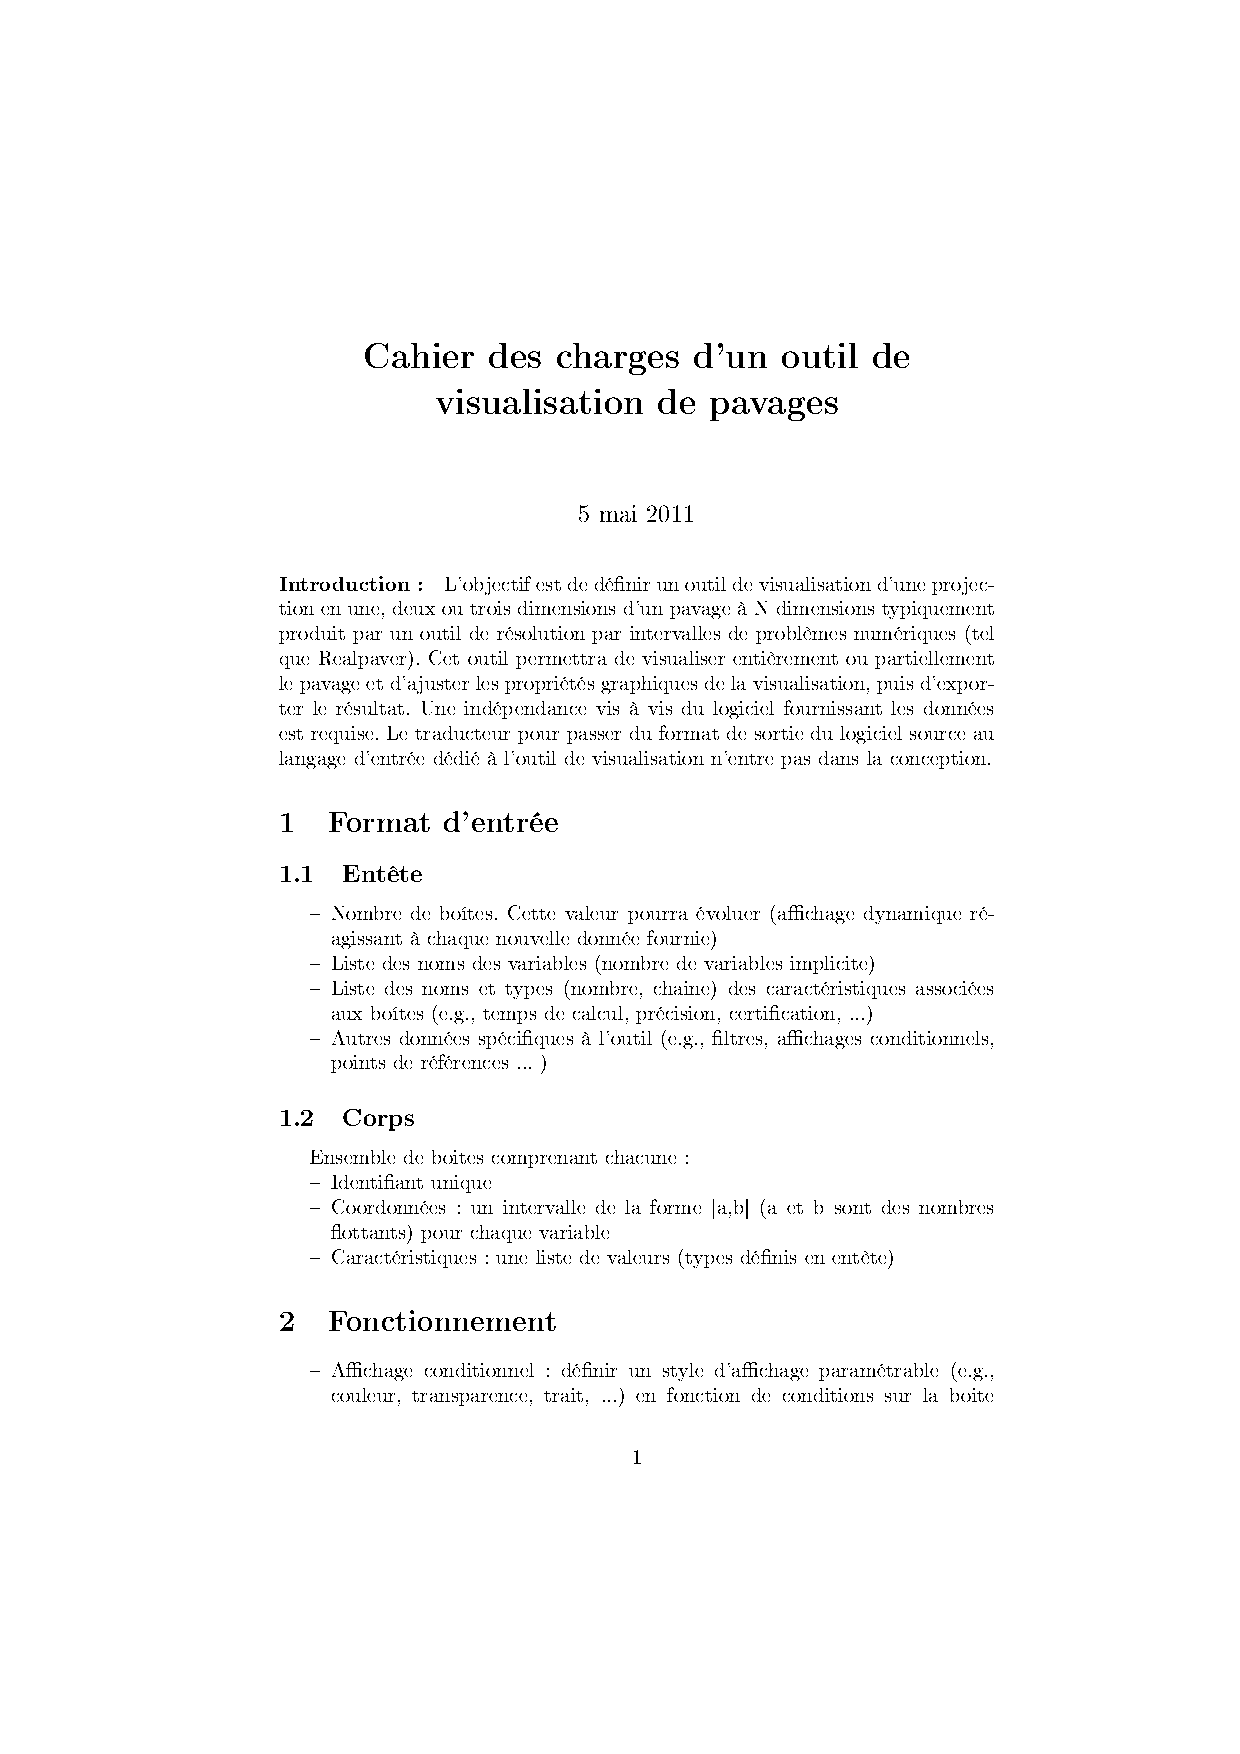
\includepdf[pages=-]{Cahier_des_charges.pdf}
\section{Documents de spéfications}\label{sec:spe}
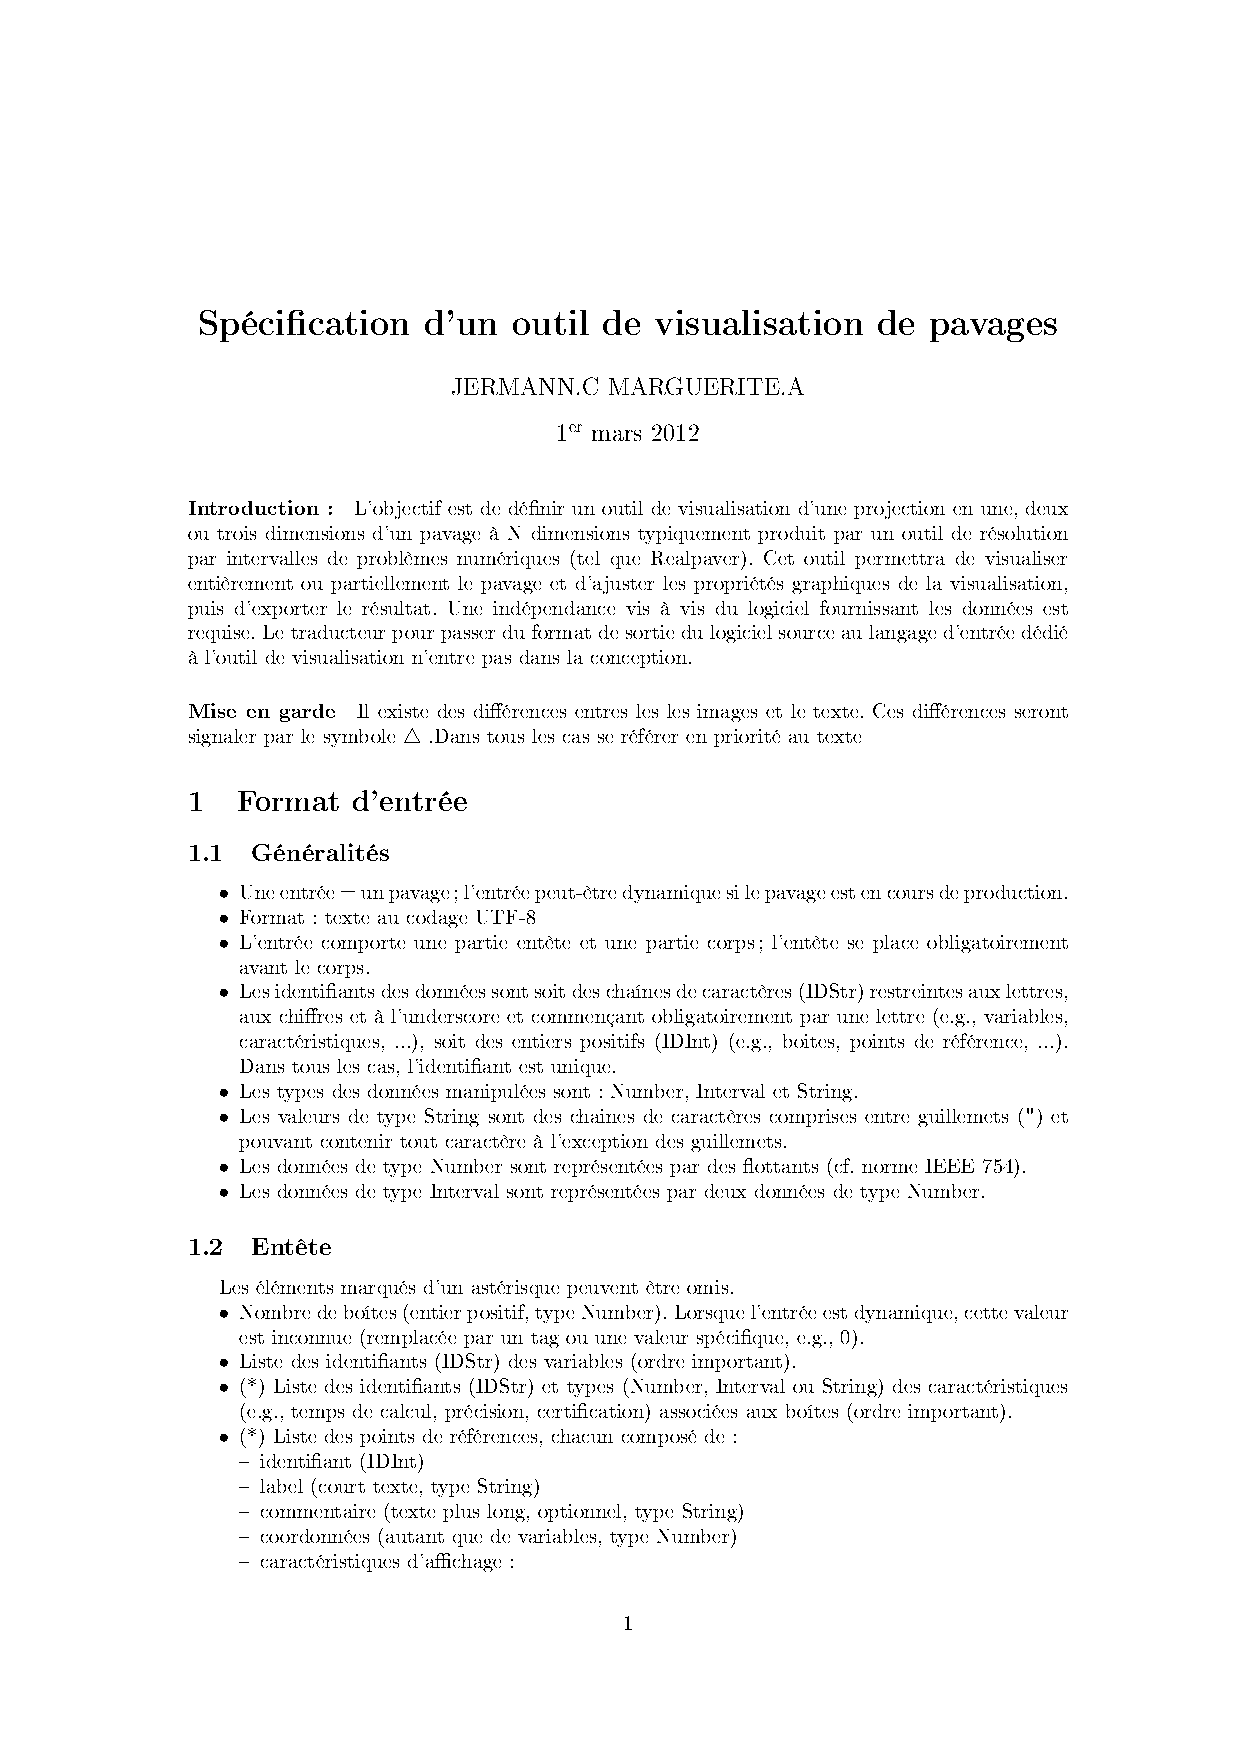
\includepdf[pages=-]{Specifications.pdf}


\listoffigures
% Pour finir l'interligne de 1,5
\bibliographystyle{alpha}
\bibliography{biblio.bib}


\end{document}
